\chapter{MẠCH CẦU H}
    \section{Cấu tạo của mạch cầu H}
        Mạch cầu H là một mạch điện tử cơ bản được sử dụng rộng rãi để điều khiển hướng quay của động cơ một chiều (DC) hoặc điều khiển công suất truyền đến tải. Hình dạng mạch khi vẽ ra giống chữ H, nên được gọi là mạch cầu H.\\
        Mạch cầu H, như tên gọi của nó, được thiết kế với cấu trúc cơ bản hình chữ H. Cấu tạo chính của mạch bao gồm: 
        \vspace{-0.4cm}
        \begin{itemize}
            \item 4 công tắc điện tử: Đây là các linh kiện chính của mạch, thường là transistor (BJT) hoặc MOSFET. Chúng đóng vai trò như những chiếc cầu nối, điều khiển dòng điện đi qua động cơ.
            \item Diode bảo vệ: Các diode được mắc song song với mỗi công tắc để bảo vệ chúng khỏi hiện tượng điện áp ngược khi các công tắc tắt.
            \item Nguồn cung cấp: Cung cấp điện áp một chiều để cấp cho mạch và động cơ.
        \end{itemize}
        \begin{figure}[H]
            \centering
            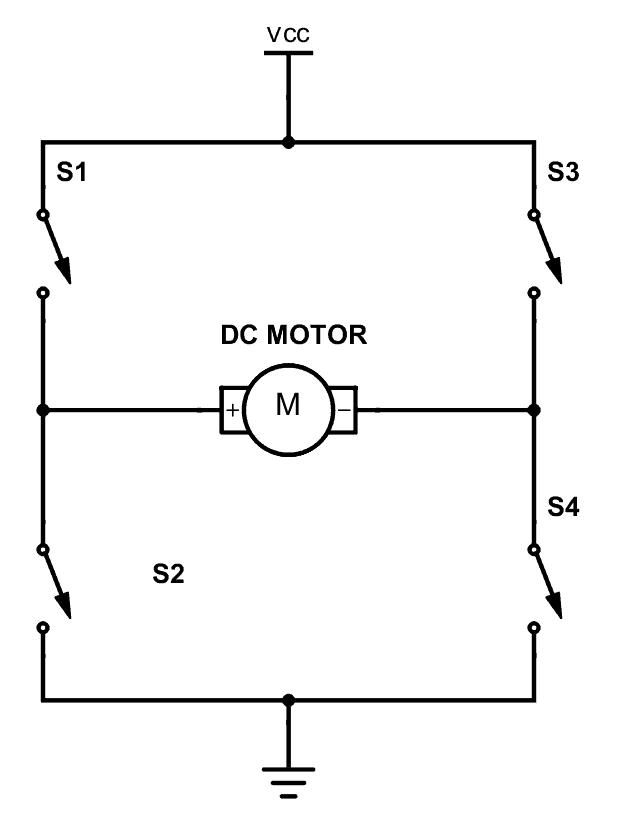
\includegraphics[width=0.4\textwidth]{pictures/cauhsimple.png}
            \caption{Mạch cầu H đơn giản}
            \label{fig:hbridge}
        \end{figure}
        \begin{figure}[H]
            \centering
            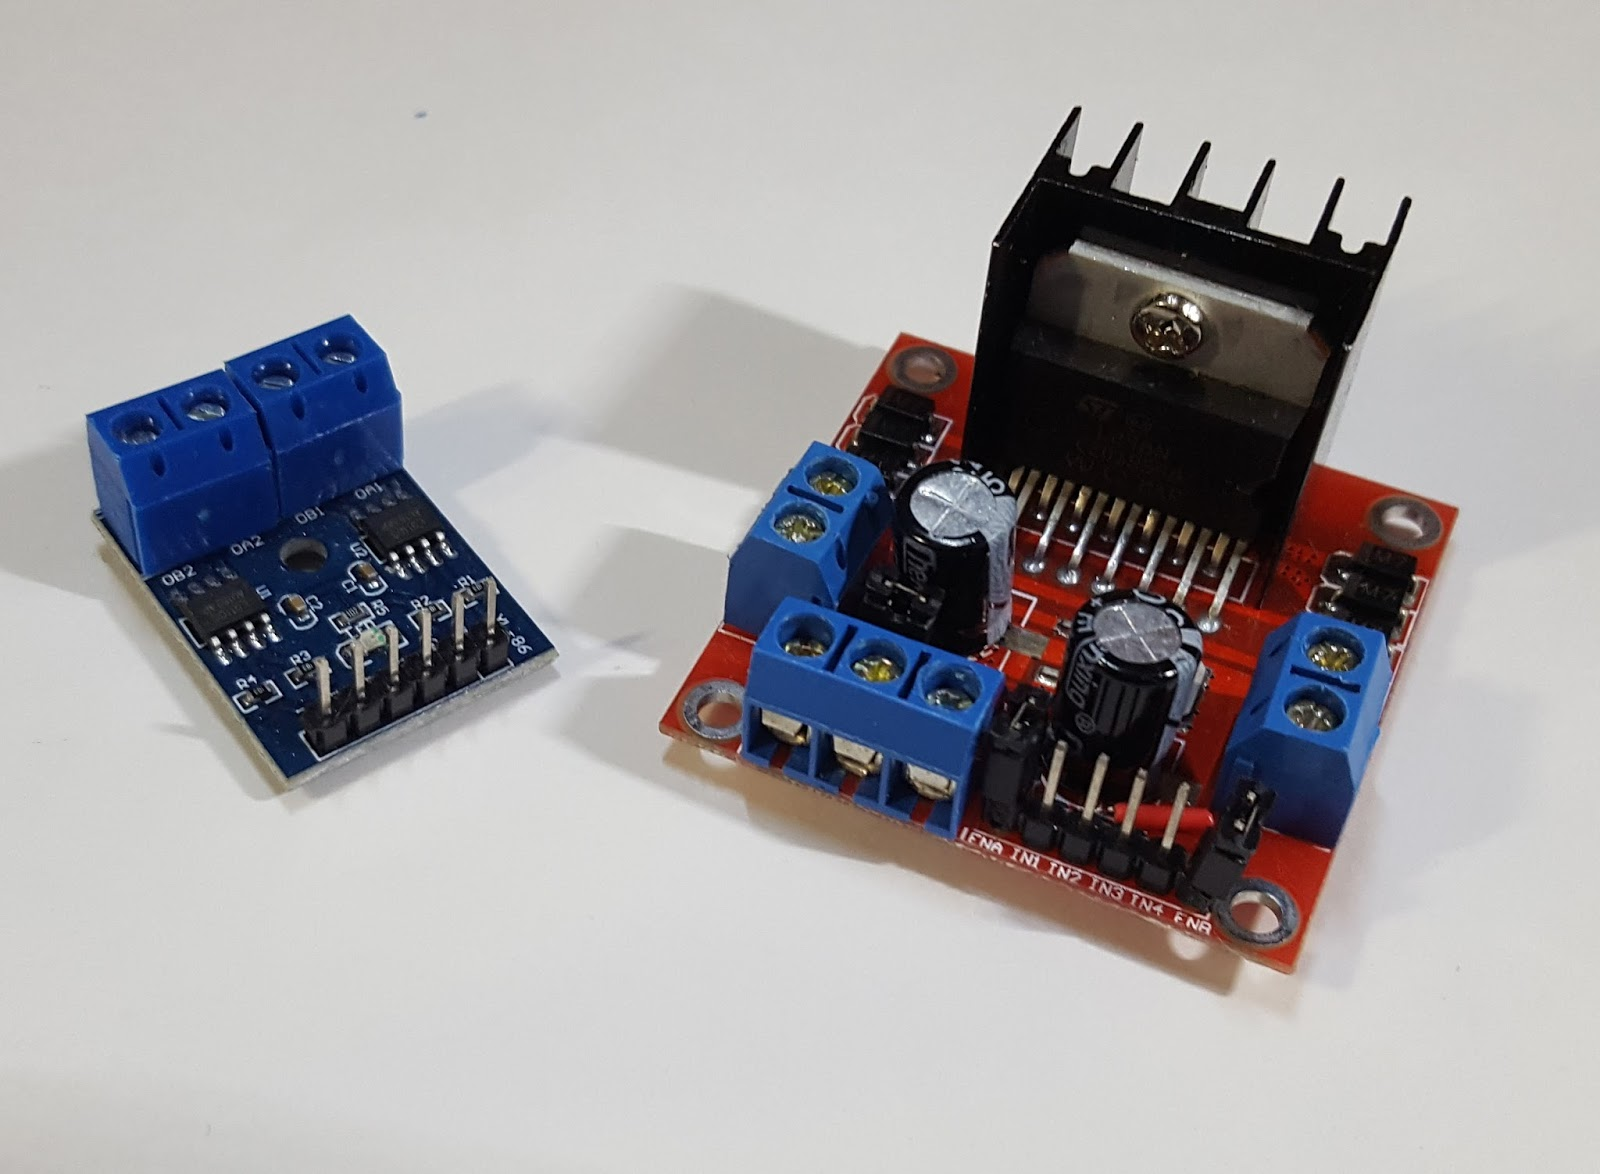
\includegraphics[width=0.5\textwidth]{pictures/cauhcurcuit.png}
            \caption{Các mô đun có tích hợp mạch cầu H}
            \label{fig:hbridge}
        \end{figure}
        \cleardoublepage
        \subsection{Nguyên lý hoạt động của mạch cầu H}
        \begin{figure}[H]
            \centering
            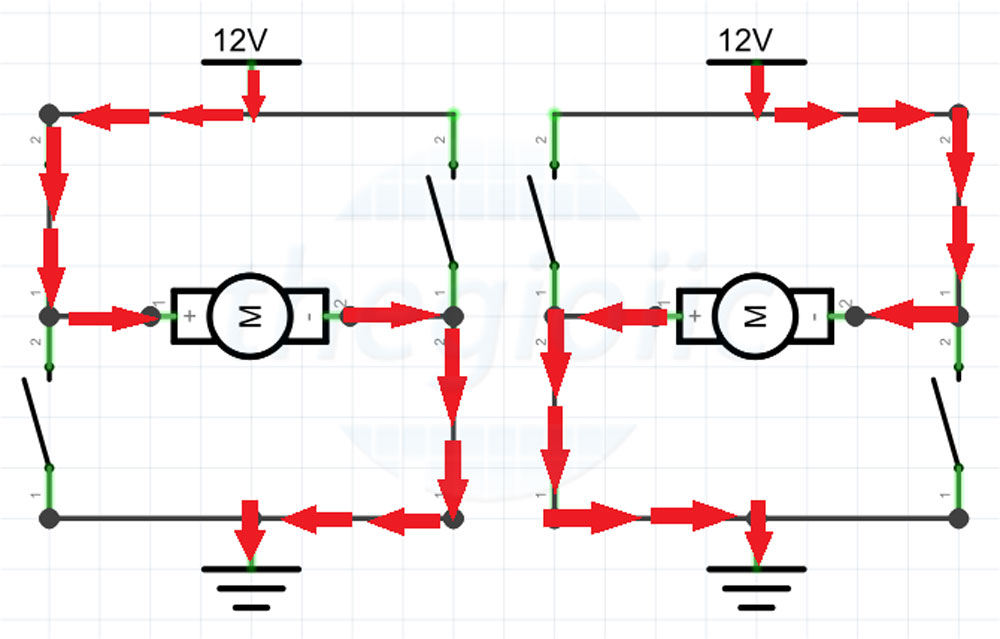
\includegraphics[width=0.8\textwidth]{pictures/cauhwork.png}
            \caption{Nguyên lý hoạt động của mạch cầu H}
            \label{fig:hbridge}
        \end{figure}
        \hspace*{0.6cm}Trong mô hình này, chúng ta sử dụng mạch cầu H để điều khiển động cơ một chiều. Động cơ DC có thể quay theo chiều thuận hoặc chiều nghịch, tùy thuộc vào cách chúng ta kết nổi cực âm và cực dương cho động cơ.

        Mạch cầu H được thiết kế để điều khiển động cơ DC hoặc tải điện theo hai hướng: hướng thuận và hướng nghịch. Mạch này bao gồm bốn transistor hoặc MOSFET được kết nối với nhau theo cấu trúc dạng cầu.

        Khi một cặp transistor được kích hoạt, một transistor ở phía trên và một transistor ở phía dưới, dòng điện sẽ chảy qua động cơ theo hướng tương ứng. Khi cặp transistor khác được kích hoạt, hướng dòng điện sẽ đảo ngược, từ đó điều khiển tải đi theo hướng khác

        Việc điều khiển được thực hiện thông qua các cổng điều khiển được kết nối đến bồn transistor hoặc MOSFET, khi điện áp được đưa vào các cổng này, các transistor sẽ được kích hoạt hoặc ngưng hoạt động tùy thuộc vào tín hiệu đầu vào tại cổng.
        \cleardoublepage
    \section{Ứng dụng mạch cầu H trong thực tế}
        Bên cạnh việc điều khiển động cơ DC, mạch cầu H còn được sử dụng rộng rãi trong các ứng dụng khác như:
        \begin{itemize}
            \item Điều khiển động cơ servo: Mạch cầu H cũng được sử dụng để điều khiển động cơ servo trong các ứng dụng yêu cầu độ chính xác cao như robotica, máy bay điều khiển từ xa và các thiết bị tự động hóa khác.
            \item Hệ thống quản lý năng lượng: Mạch cầu H được tích hợp vào hệ thống quản lý năng lượng để điều khiển việc cung cấp năng lượng cho các thiết bị điện tử như ổ đĩa động cơ, hệ thống điều hòa không khí và thiết bị gia dụng.
            \item Hệ thống truyền dẫn điện không dây: Trong các ứng dụng truyền dẫn điện không dây như sạc không dây cho điện thoại di động, mạch cầu H có thể được sử dụng để điều khiển nguồn điện được truyền từ trạm sạc đến thiết bị di động.
            \item Hệ thống giao thông thông minh: Trong các hệ thống giao thông thông minh, mạch cầu H có thể được sử dụng để điều khiển các thiết bị như cổng xoay, cửa tự động và đèn tín hiệu giao thông để tạo ra một mạng lưới giao thông hiệu quả và an toàn.
        \end{itemize}
        \begin{figure}[H]
            \centering
            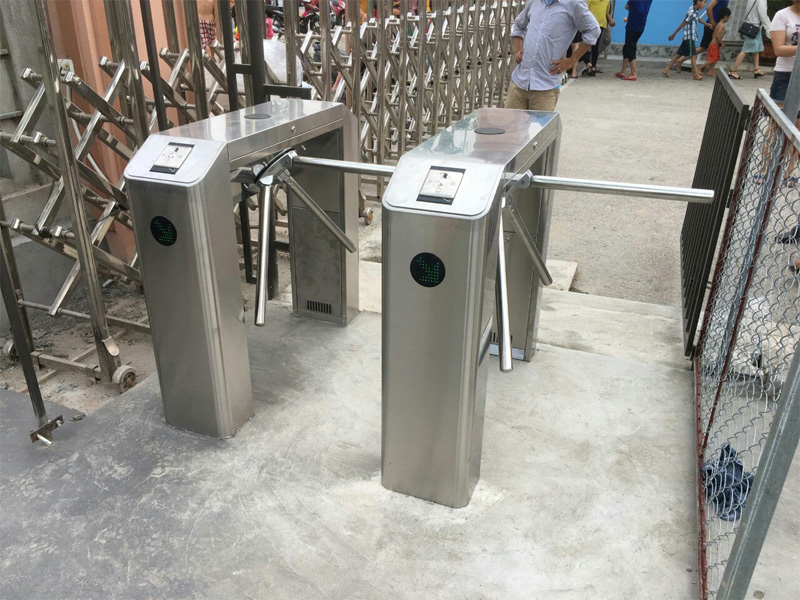
\includegraphics[width=1\textwidth]{pictures/cong3que.png}
            \caption{Hệ thống cổng xoay 3 càng có sử dụng mạch cầu H}
            \label{fig:hbridge}
        \end{figure}
        \cleardoublepage